We are interested in examining the performance of algorithms to compute minimal IVCs.  We examine three algorithms: \textbf{Offline MARCO}, the algorithm from~\cite{Ghass17AllIVCs}, \textbf{Online MARCO}, a variant of the algorithm from~\cite{Ghass17AllIVCs} that performs a shrink step prior to returning a solution to ensure minimality, and \textbf{Our New Hotness!}, the algorithm described in this paper.  We investigate the following research questions: (RQ1:) For all models, how many MIVCs are found within the timeout?  (RQ2:) For {\em complete} results, in which all MIVCs are found, how much time is required to complete the enumeration of MIVCs?  Finally, we are interested in how many solver calls are necessary for adequate and inadequate results.  Thus, we add (RQ3:) What is the (average) number of adequacy/inadequacy checks required to produce individual MIVCs?

%\emph{This RQ makes sense only for online algorithms, i.e. we compare the new algorithm and the online MARCO.}
%	\item Optionally, we can add another RQs, such as the average time required to produce individual MIVCs or the rate of the enumeration. However, we do not have much space left. Also, the three above mentioned RQs should be enough :)
%\end{enumerate}

\paragraph{Experimental Setup}:  We start from a benchmark suite that is a superset of the benchmarks used in \cite{Ghass17AllIVCs}. This suite contains 660 models, and includes all models that yield a valid result (530 in total) from previous Lustre model checking papers~\cite{Hagen08:FMCAD,piskac2016} and 130 industrial models yielding valid results derived from an infusion pump system \cite{hilt2013} and other sources \cite{piskac2016,NFM2015:backes}.
As this paper is concerned with analysis problems involving multiple MIVCs, we include only models that had more than 5 MIVCs (360 models in total).  To consider problems with many IVCs, we took the models that produced more than 20 MIVCs (7 models in total) and mutated them, constructing 20 mutants for each model.  We added the mutants that still yielded valid results (66 in total) back to the benchmark suite.
Thus, the final suite contains 426 Lustre models. The original benchmarks and our augmented benchmark are available from \cite{bench}.

For each test model, we configured \jkind\ to use the \texttt{Z3} solver and the ``fastest'' mode of \jkind\ (which involves running the $k$-induction and PDR engines in parallel and terminating when a solution is found). The experiments were run on a  3.50GHz  Intel(R) i5-4690 processor 16 GB memory machine running Linux with a 30 minute timeout.  All experimental data is available online~\cite{expr}.

%Given that we are primarily concerned with performance, we ask the following research questions:
%\subsection{Research Questions}
%\textcolor{red}{We need to give the algorithms name... choose something like OFFLINE\_AIVC, ONLINE\_AIVC, GS\_AIVC (grow-shrink)... I don't know, something that makes sense for the new algorithms ;) }
%\begin{enumerate}
%	\item How many MIVCs are found within a given timeout by individual algorithms? %\emph{This RQ makes sense only for online algorithms, i.e. we compare the new algorithm and the online MARCO.}
%	\item How much time does it take to complete the enumeration in the case of tractable benchmarks (benchmarks where all MIVCs can be found within the given timeout)? %\emph{This RQ makes sense for all the three algorithms: the new algorithm, online MARCO, and offline MARCO.}
%	\item What is the (average) number of adequacy checks required to produce individual MIVCs? %\emph{This RQ makes sense only for online algorithms, i.e. we compare the new algorithm and the online MARCO.}
%	\item Optionally, we can add another RQs, such as the average time required to produce individual MIVCs or the rate of the enumeration. However, we do not have much space left. Also, the three above mentioned RQs should be enough :)
%\end{enumerate}
%\textcolor{red}{great! I'll add the results later (tomorrow) }

%\begin{figure}[!t]
%\centering
%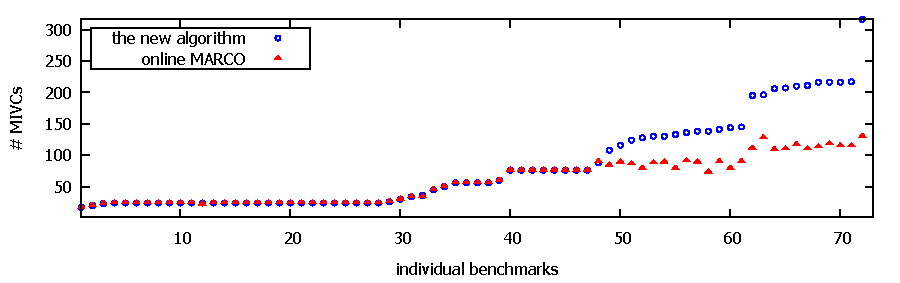
\includegraphics[scale=0.8]{./plots/found_mivcs.pdf}
%\caption{Number of produced MIVCs by online algorithms}
%\label{res:found_mivcs}
%\end{figure}
%
%\begin{figure}[!t]
%\centering
%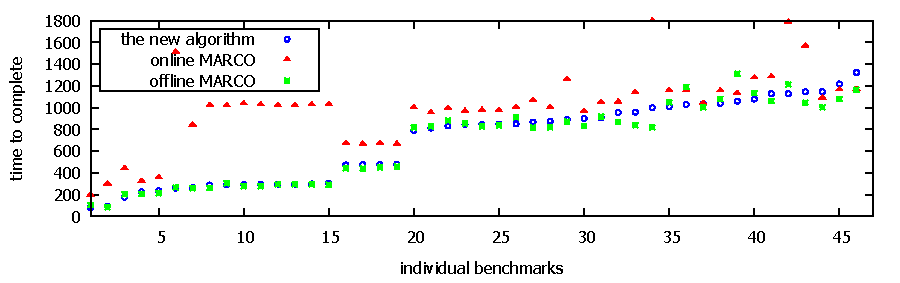
\includegraphics[scale=0.8]{./plots/time_to_complete.pdf}
%\caption{Runtime for tractable benchmarks (those that completed within the timeout)}
%\label{res:time_to_complete}
%\end{figure}



\begin{figure}
\centering
\begin{minipage}{.45\textwidth}
\centering
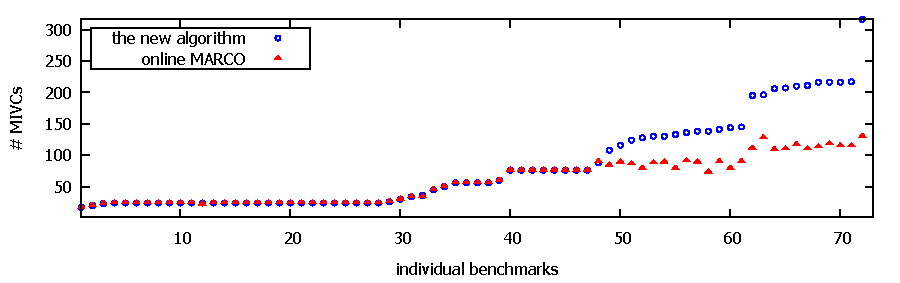
\includegraphics[scale=0.8]{./plots/found_mivcs.pdf}%
\captionof{figure}{Number of produced MIVCs\\ by online algorithms.}%
\label{res:found_mivcs}
\end{minipage}\hfill
\begin{minipage}{.45\textwidth}
\centering
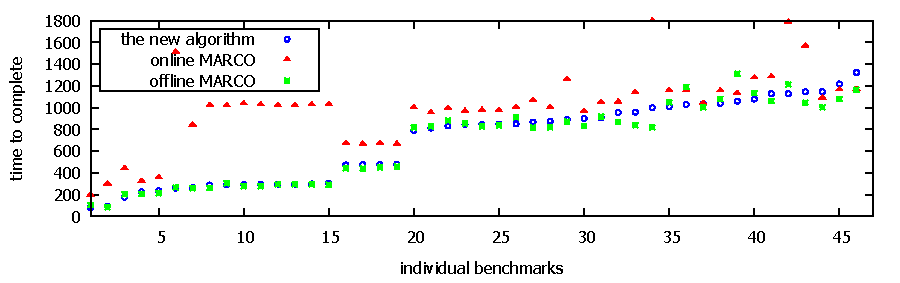
\includegraphics[scale=0.8]{./plots/time_to_complete.pdf}%
\captionof{figure}{Runtime for tractable benchmarks.}%
\label{res:time_to_complete}
\end{minipage}
\end{figure}



\begin{figure}[!t]
\centering
\begin{subfigure}{.5\textwidth}
  \centering
  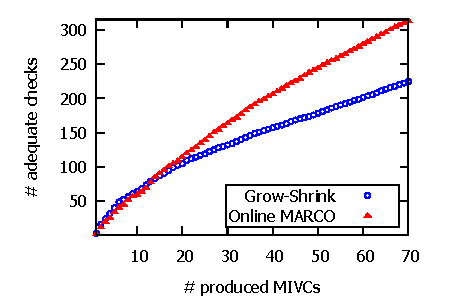
\includegraphics[scale=0.8]{./plots/adequate_checks_per_mivc_70.pdf}
  \caption{Checks with result "adequate".}
  \label{res:adequate_checks}
\end{subfigure}%
\begin{subfigure}{.5\textwidth}
  \centering
  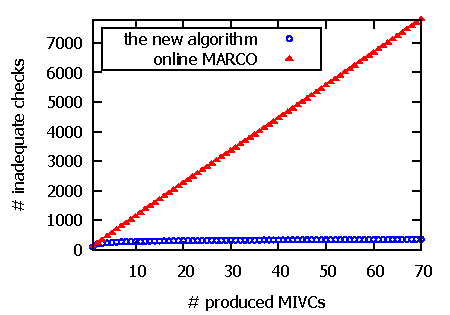
\includegraphics[scale=0.8]{./plots/inadequate_checks_per_mivc_70.pdf}
  \caption{Checks with result "inadequate".}
  \label{res:inadequate_checks}
\end{subfigure}
\caption{Average number of performed adequacy checks required to produce individual MIVCs}
\label{res:checks}
\end{figure}

\subsection{Experimental Results}
In this section, we examine the experimental results to address the research questions.

\paragraph{RQ1 an RQ2:}
Data relted to the first two research questions is shown in Figures~\ref{res:found_mivcs} and~\ref{res:time_to_complete}.  The first figure shows the number of computed MIVCs for each algorithm.  \mike{Why do we have different numbers of benchmarks for the two figures?}  Figure~\ref{res:found_mivcs} describes the number of MIVCs found for each benchmark using the two online algorithms.  For the first \mike{XXX} models, both algorithms finish within the time limit, so produce the same number of MIVCs.  For the \mike{XX} models in which both algorithms do not complete, the \mike{NAME?} algorithm substantially performs Online MARCO, finding an average of \mike{YY\%} additional MIVCs. Figure~\ref{res:time_to_complete} describes the time for each algorithm. \mike{This graph should have a log scale for time}.  We see that the performance of the \mike{NAME?} algorithm is very similar to offline MARCO, but as previously discussed, has the advantage of returning guaranteed MIVCs, rather than approximate IVCs.  It is much faster than the Online MARCO algorithm which produces MIVCs using MARCO and shrinking.

\paragraph{RQ3:}  For RQ3, we examined the number of required calls to the solver per IVC.  For this question, we used the 33 models that contained a large number of IVCs ($>$70) in order to show the solver efficiency as the number of IVCs increased.  A point with coordinates $(x,y)$ states that the algorithm needed to perform $y$ solver calls (on average) in order to produce (find) the first $x$ MIVCs. We grouped the calls in terms of the number of calls that returned {\em adequate} vs. {\em inadequate} results.  It is evidenced by the results in Figure~\ref{res:checks}, the new algorithm improves upon online MARCO as the number of MIVCs becomes larger. 

The improvement in the number of \emph{inadequate} calls is due the novel shrinking and growing procedures. 
Each (approximately) maximal inadequate subset found by the growing procedure allows to save (up to exponentially) many inadequate calls during subsequent executions of the shrinking procedure.
Indeed, the new algorithm performed on average only 353 inadequate calls to output the first 70 MIVCs, whereas the online MARCO needed to perform 7775 calls to output the same number of MIVCs. 

The improvement in the number of adequate calls is not so significant as in the case of inadequate calls. Yet, since the adequate calls are usually much more time consuming than inadequate ones, even a slight saving in the number of adequate calls might significantly speed up the whole computation. The new algorithm saves adequate calls due to the usage of the shrinking queue and due to the invariants that are maintained by the queue. In particular, shall two comparable sets appear in the queue, only the smaller is left. Thus, the algorithm avoids shrinking of relatively large sets and saves some adequate calls.

%\mike{Do we need an explanation as to why here?}
%\mike{Can we get Figure 4(b) on a log scale, so that we get better insight into the number of calls for the new algorithm?}


%Figure~\ref{

%\textcolor{blue}{Elaheh: We should note, that the online MARCO needs to perform about the same number of adequacy checks in order to find individual MIVCs. On the other hand, in the case of the new algorithm, the number of adequacy checks required to output each subsequent MIVC is decreasing. In particular, the new algorithm needs to perform almost no "inadequate" checks (this is caused by our novel efficient shrink procedure). Also, our algorithm needs to perform less adequate checks. We have observed, the rate of the enumeration of MIVCs of the online MARCO is stable. On the other hand, the new algorithm is getting faster with each subsequent MIVC since it needs to perform less and less adequacy checks. Therefore, the larger timeout we set (for intractable benchmark), the bigger is the improvement of the new algorithm to the online MARCO.}

%\textcolor{blue}{We shall also note, that the "inadequate" checks are usually cheaper/faster then the "adequate" checks (since the former requires to find a counter-example whereas the latter requires to establish a proof). However, the exact ratio between the price of "adequate" and "inadequate" checks differs for different types of benchmarks. Our algorithm is better than online MARCO both in the number of "inadequate" as well as "adequate" checks. Yet, the improvement is more significant in the case of "inadequate" checks. Therefore, the more expensive are the "inadequate" checks for a given benchmark, the bigger is the improvement of our algorithm to the online MARCO.   }

